\documentclass{article}
\usepackage{pdfpages}
\usepackage{graphicx}
\parindent=0pt
\usepackage{float}
\usepackage{geometry}
\geometry{margin=1in}

\usepackage{Sweave}
\begin{document}
\Sconcordance{concordance:writeUpTreespotters.tex:writeUpTreespotters.Rnw:%
1 137 1 50 0}


% <><><><><><><><><><><><><><><><><><><><><><><><><><><><><><><><><><><><><><><>
\title{Short write up of the tree ring data for the Tree Spotters}
\author{Christophe}
\date{\today}
\maketitle
% <><><><><><><><><><><><><><><><><><><><><><><><><><><><><><><><><><><><><><><>

% <><><><><><><><><><><><><><><><><><><><><><><><><><><><><><><><><><><><><><><>
\section{How we collected the cores, processed, scanned and measured them}
% <><><><><><><><><><><><><><><><><><><><><><><><><><><><><><><><><><><><><><><>
\subsection{Tree coring at the Arboretum}
At the end of April 2025, Lizzie, my PhD colleague, Mao and I went to the Arboretum to core the trees the Tree Spotters have been monitoring for the last nine years (Figure \ref{fig:corearbor}). Despite the fact that coring has very little effect on the tree health, we couldn't core some trees which were mostly American beech. Fifty trees were accepted in the proposal! \\

\begin{figure}[H]
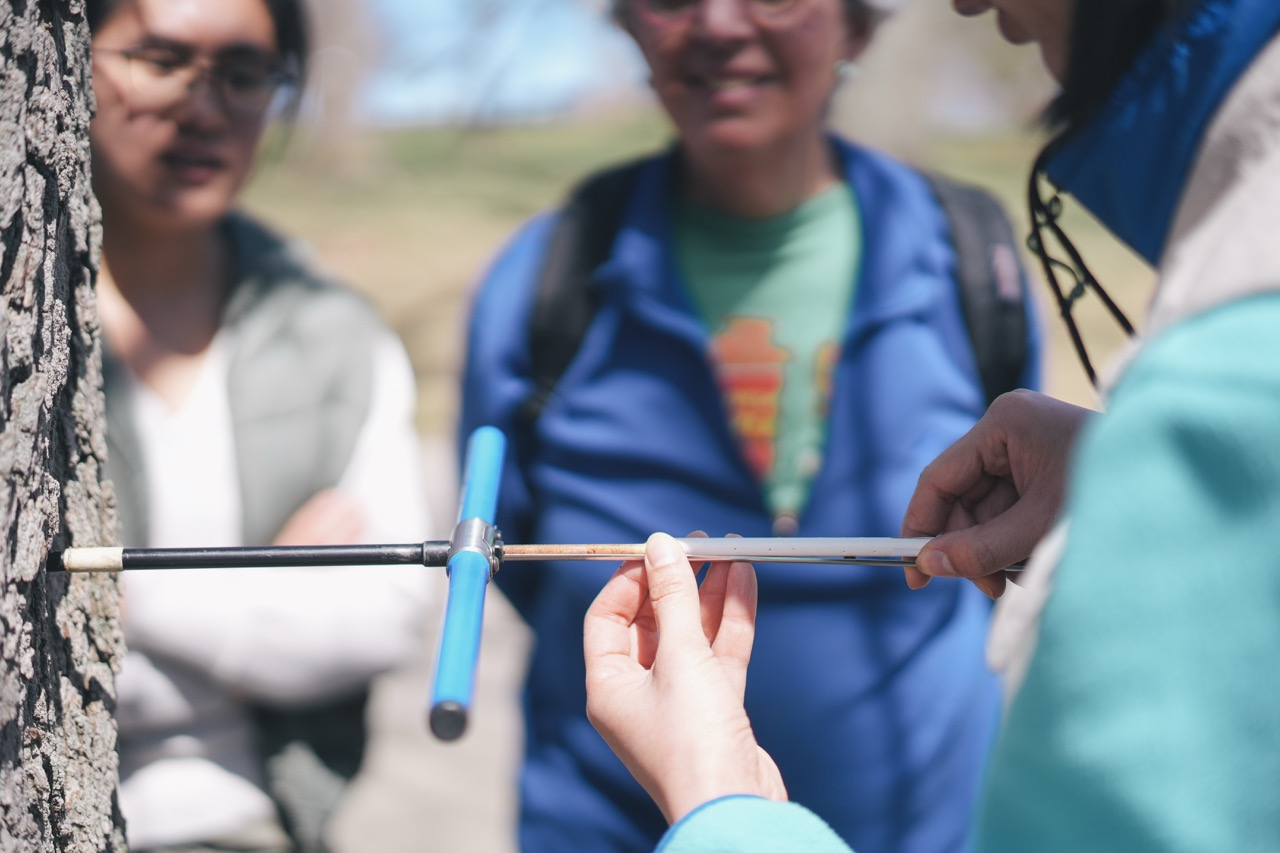
\includegraphics[width=0.8\textwidth]{photos/20250420-CRD09559lowres.jpeg}
\caption{Mao extracting a core from a White oak}
\label{fig:corearbor}
\end{figure}

During the three days coring the trees took, we had the chance to present our work and project objectives to the Tree Spotters (Figure \ref{fig:coring}). This presentation was particularly great because the Trespotters shared their experience and anecdotes with their trees that they have been monitoring for years (Figure \ref{fig:bud})!

\begin{figure}[H]
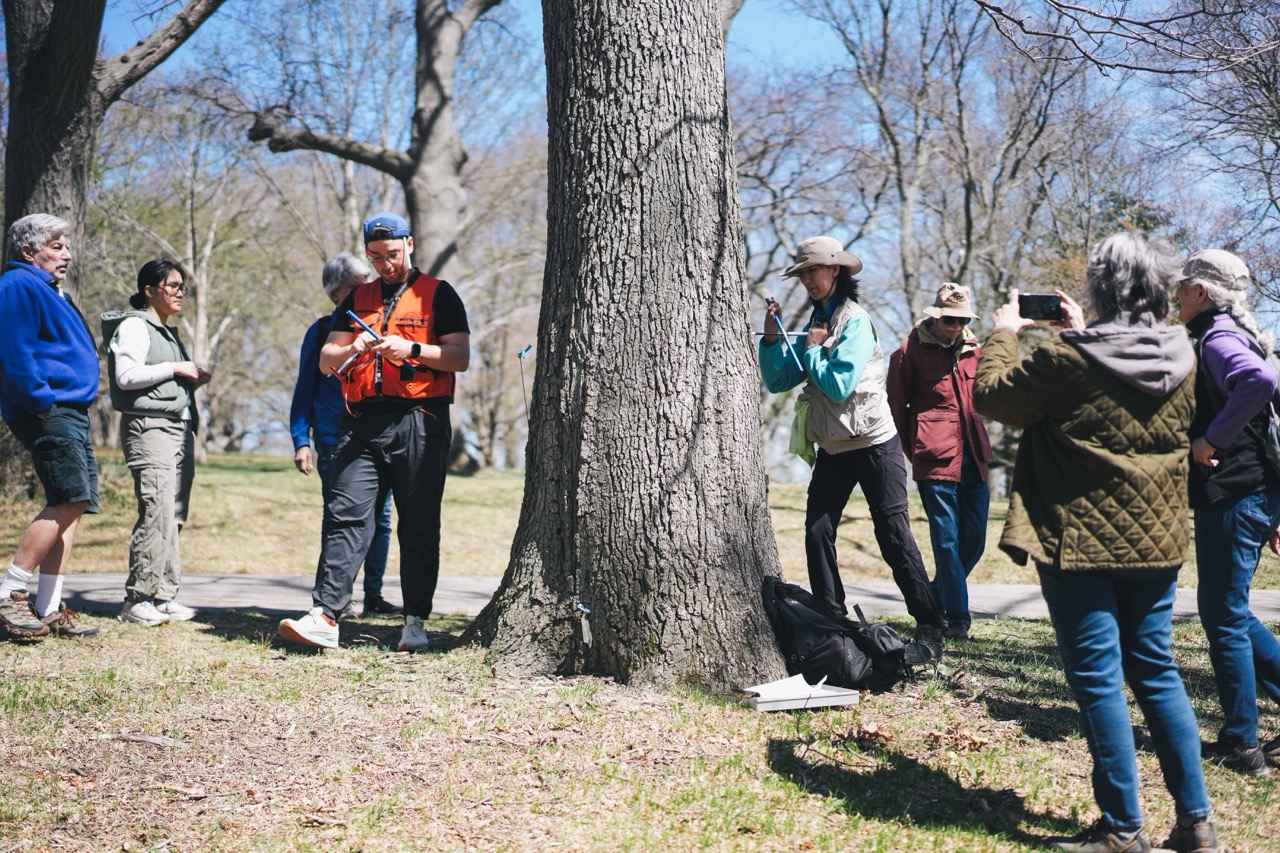
\includegraphics[width=0.9\textwidth]{photos/20250420-CRD09530_lowres.jpeg}
\caption{Mao and Christophe coring a White oak during a short presentation with the Tree Spotters}
\label{fig:coring}
\end{figure}

\begin{figure}[H]
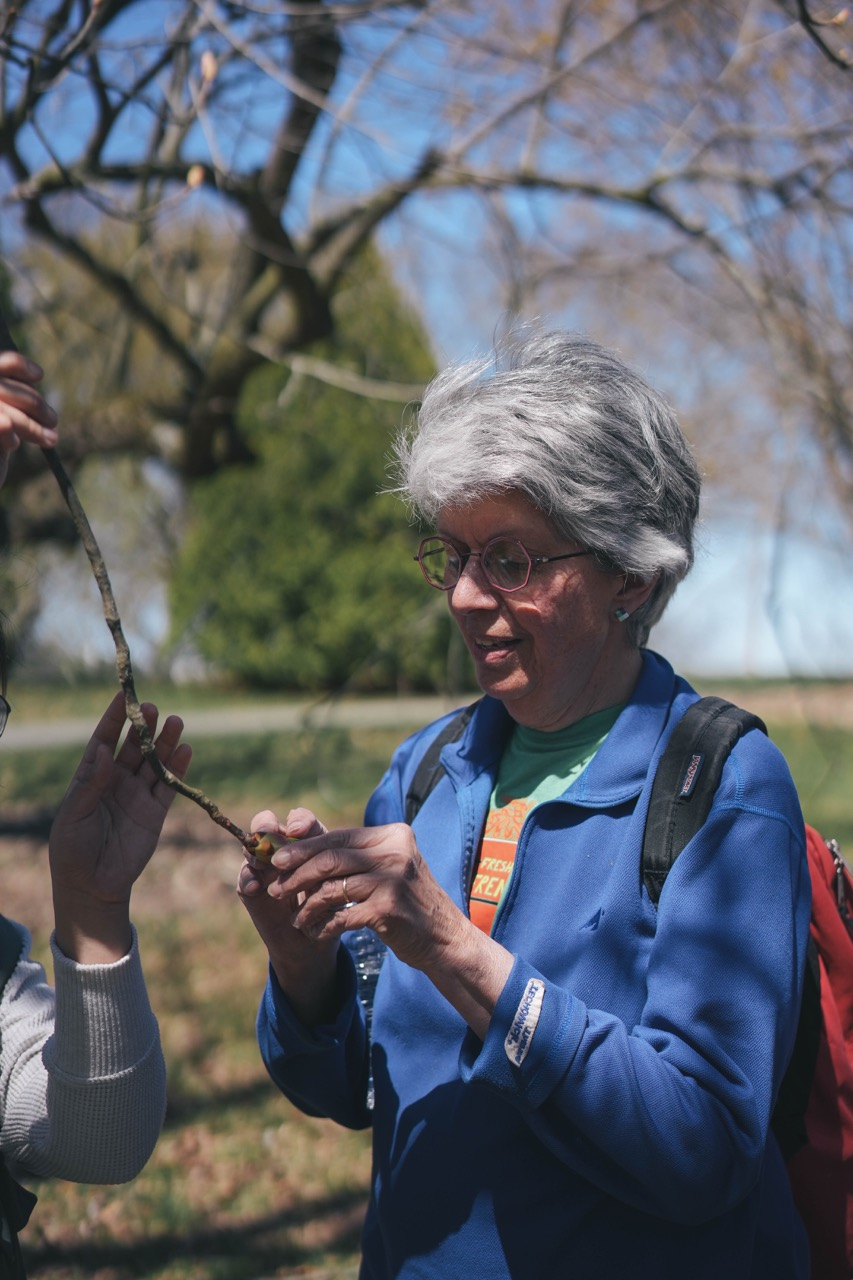
\includegraphics[width=0.6\textwidth]{photos/20250420-CRD09515lowres.jpeg}
\caption{Shanon H. looking at an early emerging bud}
\label{fig:bud}
\end{figure}

\subsection{Core mounting and sanding}
Once all the cores were collected, they were left to dry at the Weld hill building. In July, I went to pick them up so I could proceed with mounting them. We mount the tree cores on a small wooden structure to straighten the core, and also to avoid breaking it. Then I sanded the cores from a rough to a progressively finer grit, which exposes the rings nicely (Figure \ref{fig:sanding})

\begin{figure}[h!]
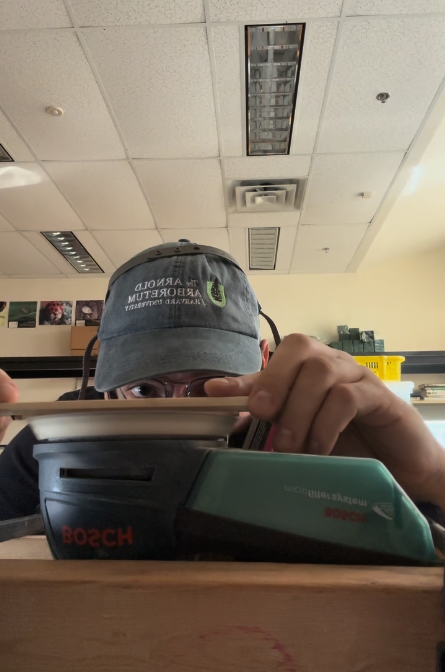
\includegraphics[width=0.4\textwidth]{photos/sanding.png}
\caption{Christophe sanding a core.}
\label{fig:sanding}
\end{figure}

\subsection{Core scanning and ring measurements}
Once all the cores were properly sanded, I scanned them at a very high resolution using our lab-made tree-ring imaging machine (TIM), that our undergraduate students created. This device has a microscopic lens attached to it that allows us to zoom in a lot onto the core to measure the ring width (Figure \ref{fig:tina}). With these cores scanned, I was able to measure each ring width for each core on my computer (Figure \ref{fig:corescan}). 

\begin{figure}[H]
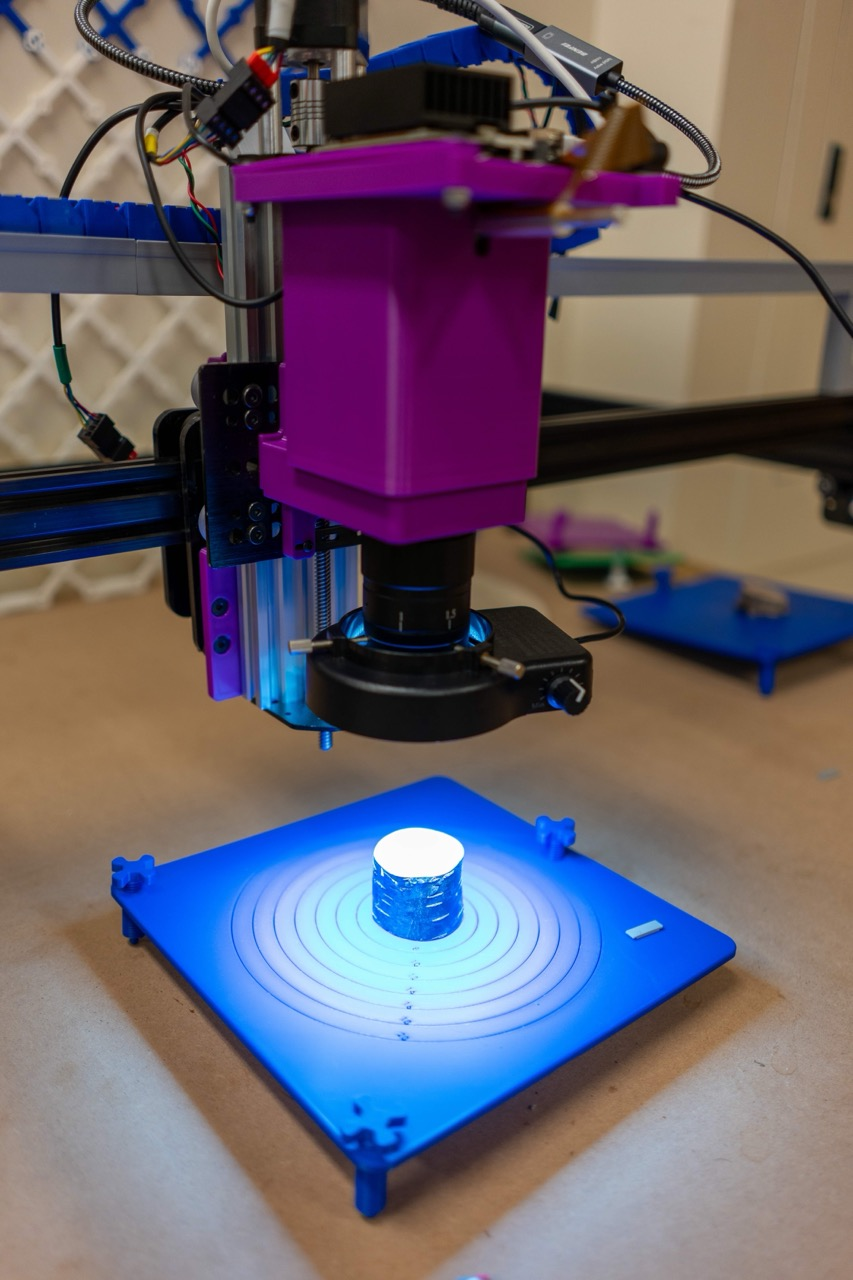
\includegraphics[width=0.6\textwidth]{photos/DSC01153lowres.jpeg}
\caption{The lab-made tree-imaging machine that we used to scan the cores}
\label{fig:tina}
\end{figure}

\begin{figure}[H]
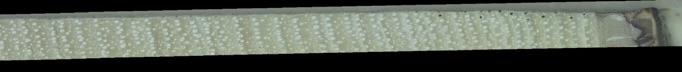
\includegraphics[width=\textwidth, height=2cm]{photos/CAOV_12907_D_ILarge2.jpeg}
\caption{An example of the scanned cores look like when I measured them. This is CAOV 12907*D.}
\label{fig:corescan}
\end{figure}

\subsection{Crossdating}
Dendrochronoly is the study of tree rings. In that field, statistical crossdating is standard and consists of dating the tree rings to the exact calendar year by comparing a chronology to other chronologies. Often, marker years are used because they represent a particularly narrow ring which can be the result of a severe drought or pest outbreak. However, statistical crossdating requires a sufficient number of trees of the same species, and a chronology at least 50 years old. These criteria were often not met with our cores. Thus, Neil Pederson and I chatted about this and decided it will be hard to perform statistical cross dating on those cores. We ended up only visually cross-dating which consists of visually matching the years across the cores of the same species (Figure \ref{fig:spagTiam}).

\begin{figure}[H]
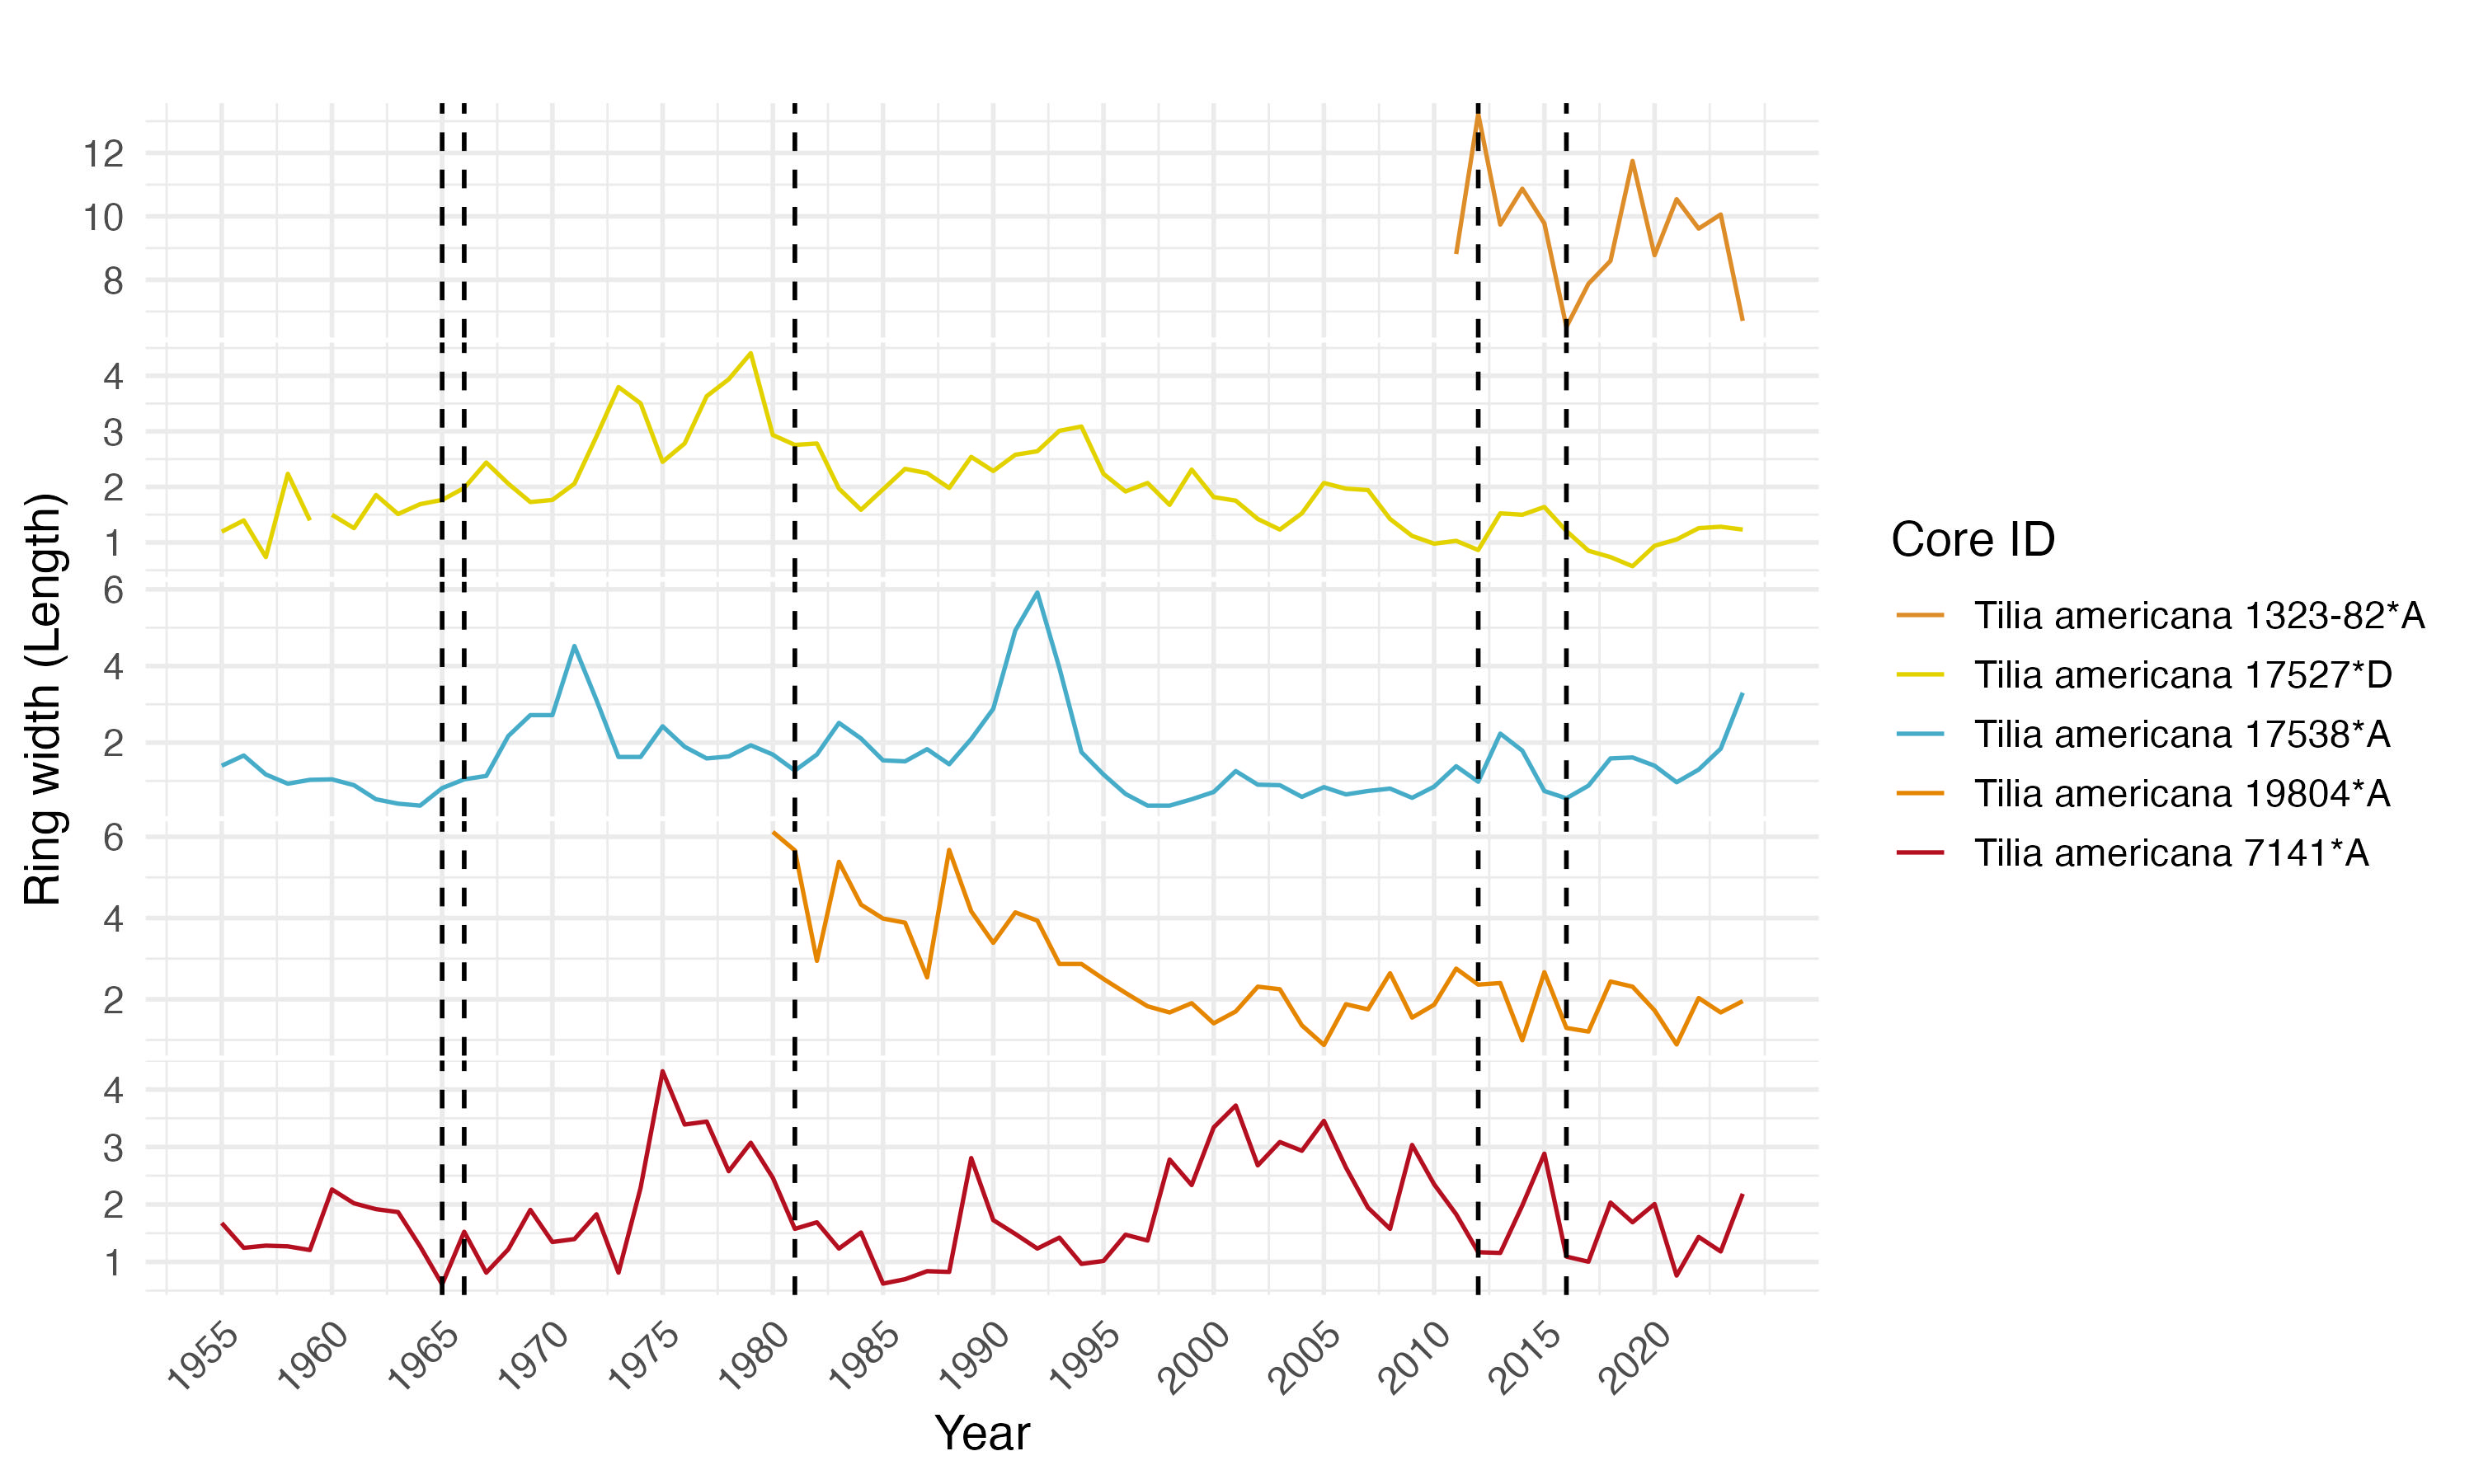
\includegraphics[width=0.9\textwidth]{../analyses/figures/tiamspaghetti_plot.jpeg}
\caption{Example of what visual crossdating looks like. This is all the American basswood (\textit{Tilia americana} chronologies that we had. The dashed lines represent marker years, for which our trees did not appear to respond to.}
\label{fig:spagTiam}
\end{figure}

% <><><><><><><><><><><><><><><><><><><><><><><><><><><><><><><><><><><><><><><>
\section{Phenology and tree-ring results}
% <><><><><><><><><><><><><><><><><><><><><><><><><><><><><><><><><><><><><><><>
With climate change, trees are shifting their phenology earlier in the spring and later in the autumn, thus extending the growing season. This is is widely expected to increase tree growth, with important effects on forest carbon sequestration dynamics. Multiple recent studies, however, have failed to find this relationship. Therefore, we will address this decoupling by using the data collected by the Tree Spotters which will allow us to investigate how the timing of phenological events affects growth across years for mature trees. We will do this by relating these observations to tree rings. We hope our results will provide a better understanding of the recently observed decoupling between growth increment and longer growing seasons.

\subsection{Phenology plots}
We plotted the two phenophases we used to calculate the growing season conditions: leafout (Figure \ref{fig:leafout}) and leaf colouring (Figure \ref{fig:coloredleaves}).

\begin{figure}[H]
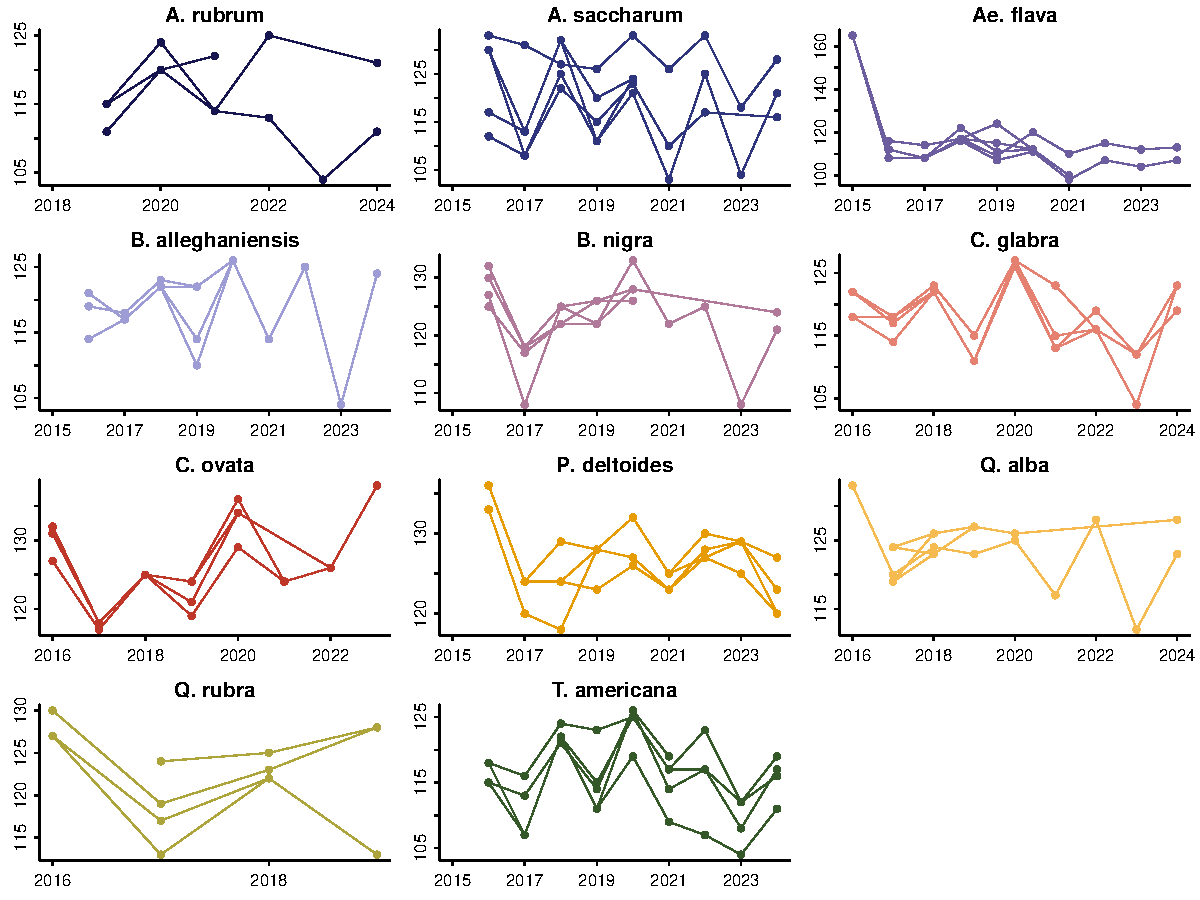
\includegraphics[width=1\textwidth]{../analyses/figures/empiricalData/leafoutXyear.pdf}
\caption{All the leafout dates recorded over the years, for each individual tree. The vertical axes represents the day of year of that observation}
\label{fig:leafout}
\end{figure}

\begin{figure}[H]
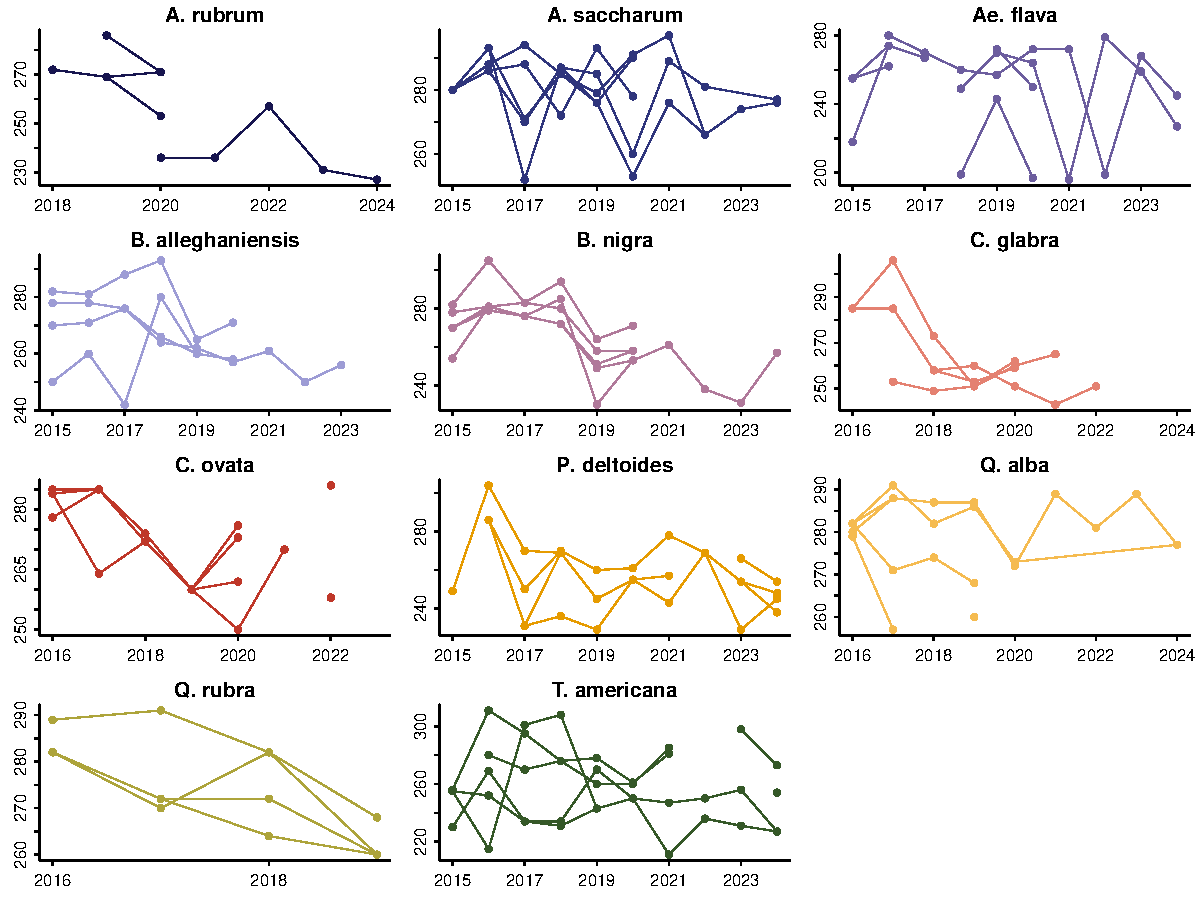
\includegraphics[width=1\textwidth]{../analyses/figures/empiricalData/coloredLeavesXyear.pdf}
\caption{All the leaf colouring dates recorded over the years, for each individual tree. The vertical axes represents the day of year of that observation}
\label{fig:coloredleaves}
\end{figure}

\subsection{Tree ring chronologies}
We present the tree-ring width as a function of year, only for the years the Tree Spotters collected phenological data for (Figure \ref{fig:rwPhenoyears}).

\begin{figure}[H]
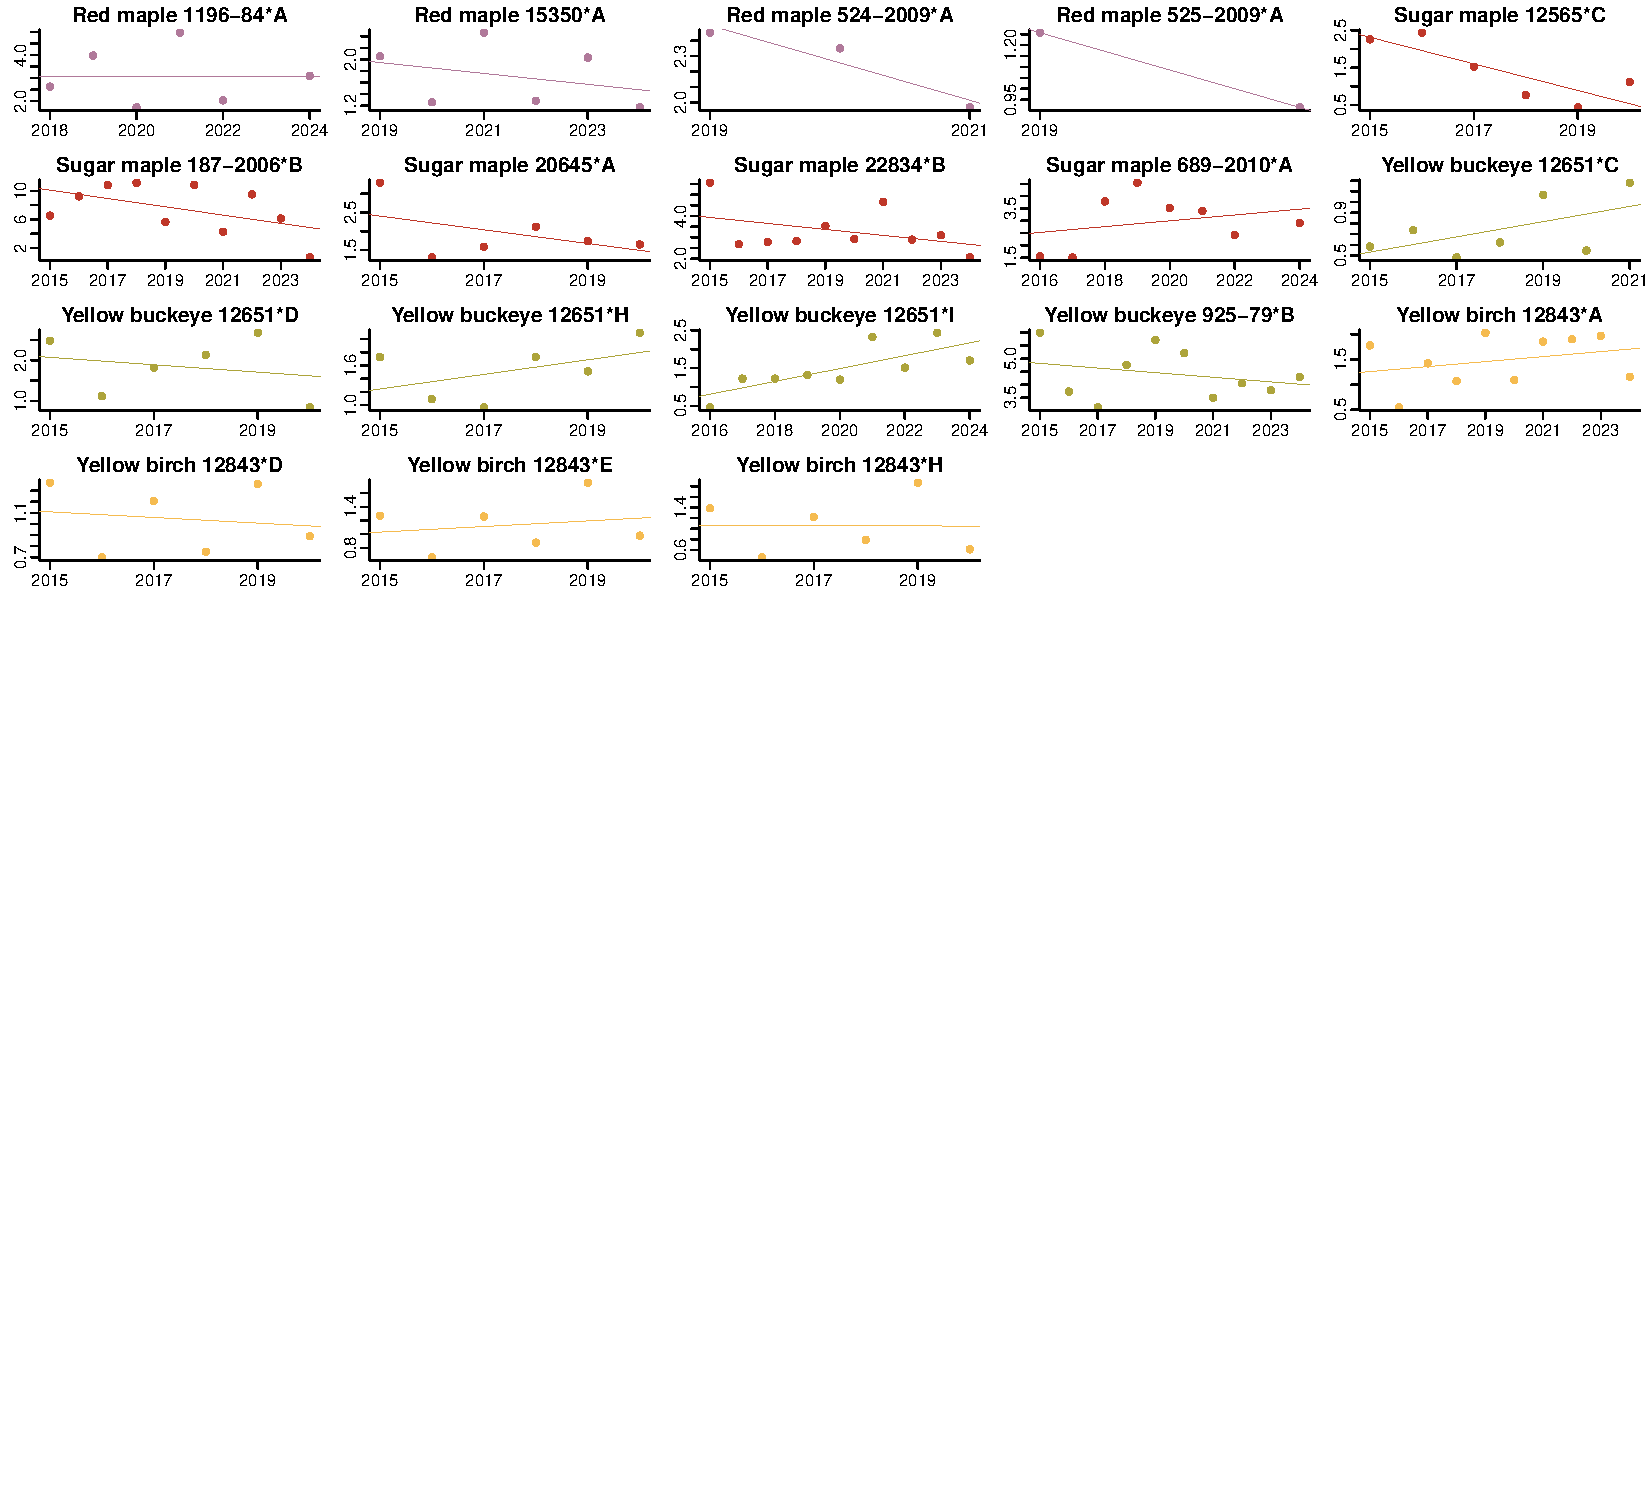
\includegraphics[width=1\textwidth]{../analyses/figures/empiricalData/ringwidthXyearPhenoData1page.pdf}
\caption{The ring width measurements as a function of each year, for each individual tree and years we have phenological observations for. The vertical axes represents the ring width of that individual.}
\label{fig:rwPhenoyears}
\end{figure}

\subsection{Preliminary results}
Our results indicate that while some species, like maples (\textit{Acer saccharum} and \textit{Acer rubrum}), River birch (\textit{Betula nigra}) and White oak (\textit{Quercus alba}) appear to grow more with increasing growing degree days (a measure of heat accumulation), others like Yellow buckeye (\textit{Aesculus flava}), Yellow birch (\textit{Betula alleghaniensis}), hickories (\textit{Carya ovata} and \textit{Carya glabra}) and American basswood (\textit{Tilia americana}) grew less. The growth of the other species was not affected by growing degree days (Figure \ref{fig:model}).

\begin{figure}[H]
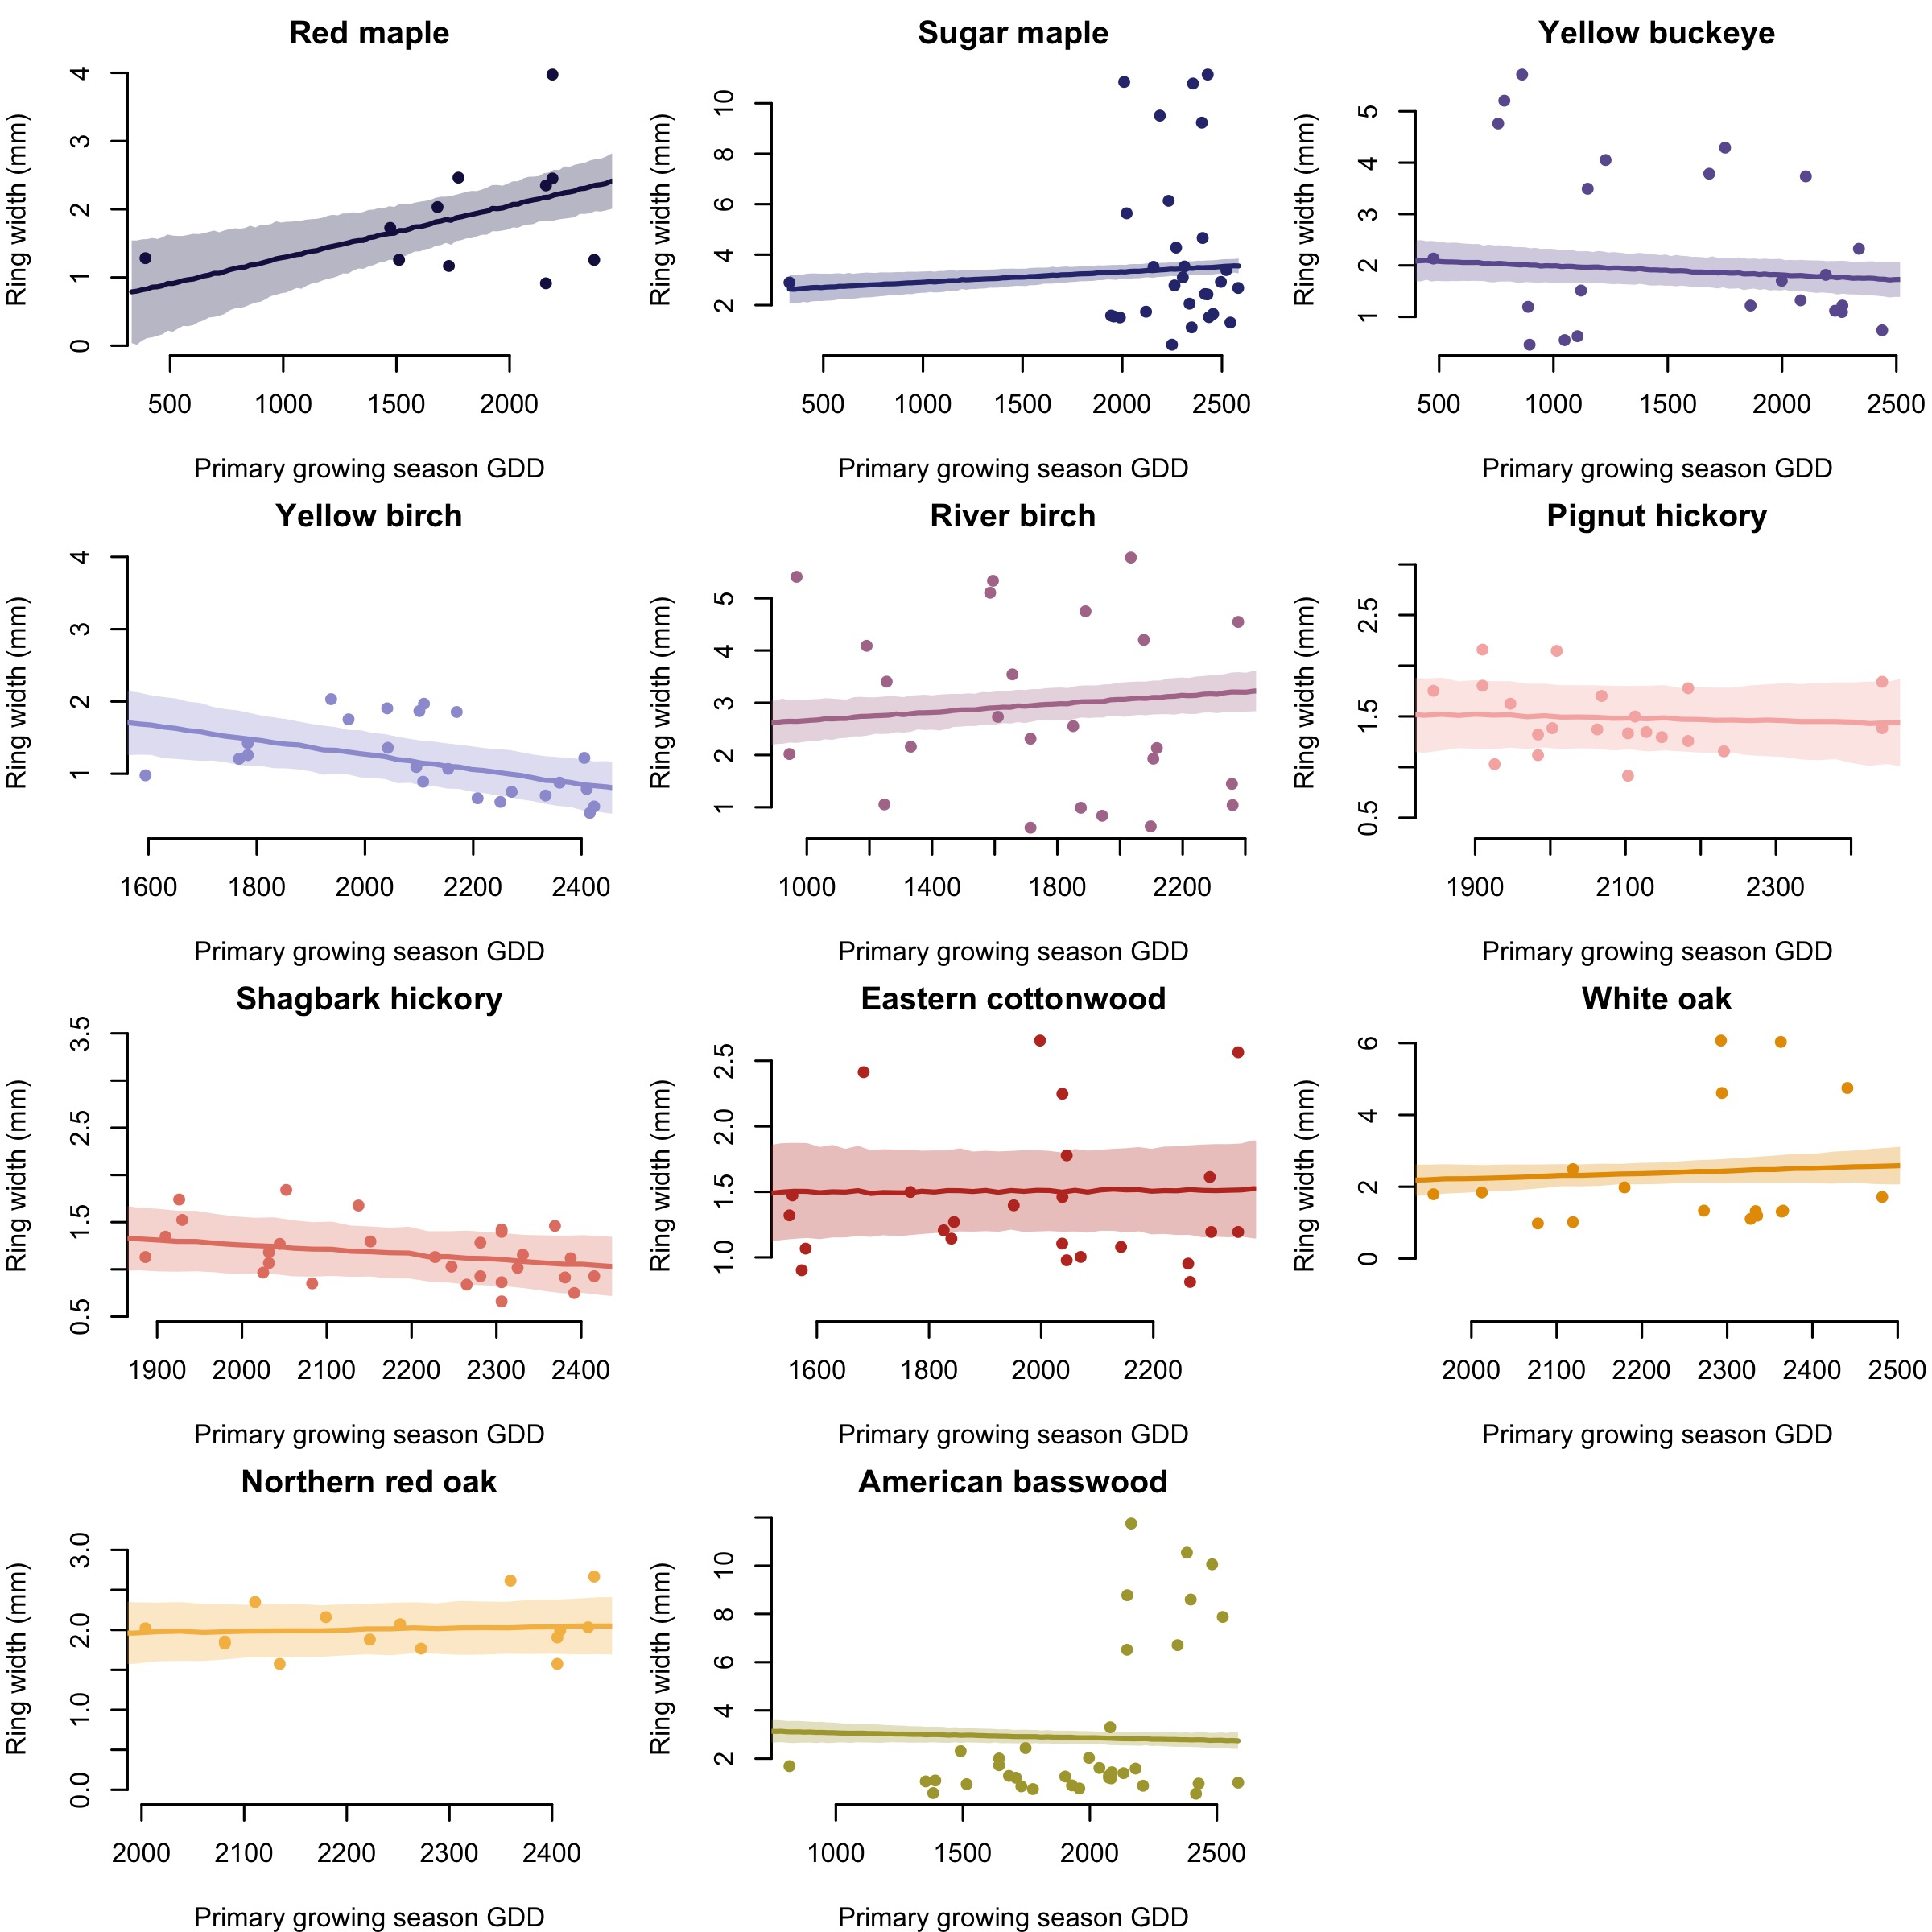
\includegraphics[width=1\textwidth]{../analyses/figures/empiricalData/growthModelSlopesperSppFacet.jpeg}
\caption{Model estimates for each species. We ran a model to estimate the ring width as a function of growing degree days (a measure of heat accumulation) for the growing season defined between leaf color date and leafout. The very low growing degree day values for Red maple (15350*A, 2022), Sugar maple (22834*B, 2022) and Yellow buckeye (12651*D
, 2018) are the result of a very early leaf coloring observation in early June.}
\label{fig:model}
\end{figure}

\section{Supplemental material}

\subsection{All the tree chronologies with a five-year averaged growing degree days}

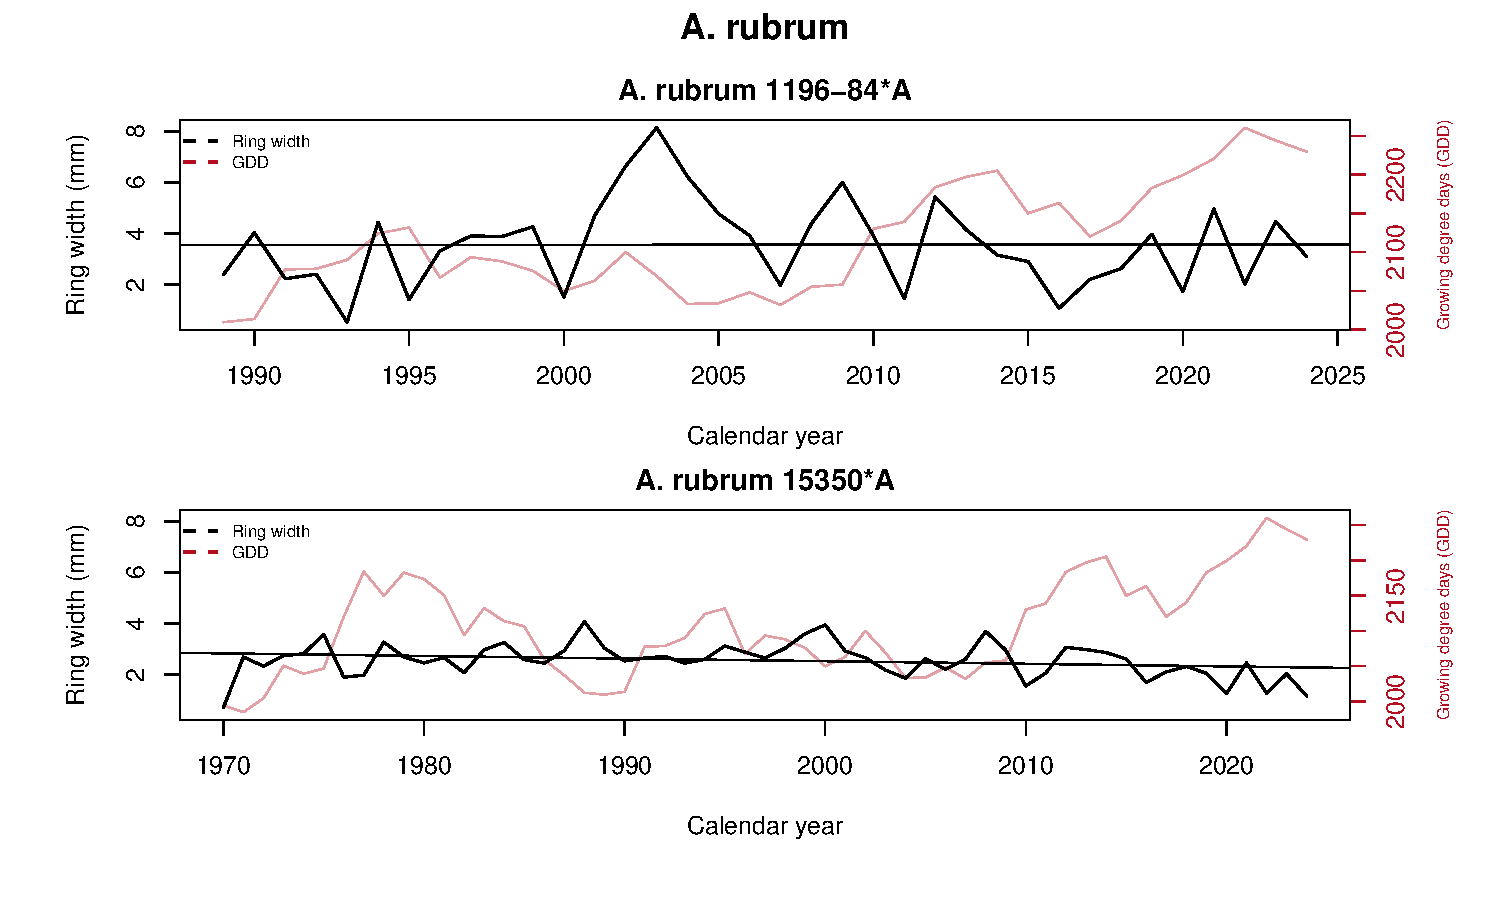
\includepdf[pages=1-10]{../analyses/figures/empiricalData/ringwidthXyear_bySpeciesAllYrs.pdf}
% \includepdf[pages=6-11]{../analyses/figures/empiricalData/ringwidthXyear_bySpeciesAllYrs.pdf}

\end{document}
